\documentclass[11pt,a4paper]{article}
\usepackage{a4wide,ngerman,url,graphicx}
\usepackage[utf8]{inputenc}

\parskip4pt
\parindent0pt


\title{Jugendstadtplan Leipzig -- technische Dokumentation}
\author{Leipzig Data Projekt}
\date{Version vom 18. Februar 2015}

\begin{document}
\maketitle

\section{Hintergrund}

Die folgende Beschreibung dokumentiert die Überarbeitung der Kartendarstellung
des Jugendstadtplanprojekts, die von einem studentischen Projektteam im Rahmen
des Interdisziplinären Moduls „Kreativität und
Technik“\footnote{\url{http://bis.informatik.uni-leipzig.de/de/Lehre/Graebe/Inter}}
im Sommersemester 2013 erstellt wurde. 

Die ursprüngliche Kartendarstellung wurde von Emanuel Ott (Student im Bachelor
Afrikanistik) im Sommersemester 2013 auf der Basis von
CloudMade\footnote{\url{http://cloudmade.com/}} erstellt.  CloudMade hat seinen
kostenfreien Kartenservice allerdings zum Mai 2014 eingestellt\footnote{„In
  March 2014 we announced that as of May 1st 2014 CloudMade will be
  discontinuing service of Map Tiles, Geocoding, Routing and Vector Stream
  Server APIs. We will provide only Map Tiles API for Enterprise users.“
  \url{http://support.cloudmade.com/}}.

Ziel der Überarbeitung war es, neben der Herstellung von Konnektivität zu einem
anderen Kartenprovider die Website auf der Basis des Web-Frameworks
\emph{Bootstrap}\footnote{\url{http://getbootstrap.com/}} neu aufzubauen sowie
die Datenschicht über die PHP-Bibliothek
\emph{EasyRDF}\footnote{\url{http://www.easyrdf.org/}} anzubinden und damit ein
prototypisches Beispiel zu schaffen, wie Webseiten mit Kartendarstellungen von
geolokalen RDF-basierten Informationen aufgebaut werden können.

Die Überarbeitung wurde durch Immanuel Plath (Student im Master Informatik) im
Wintersemester 2014/15 im Rahmen eines Praktikumsauftrags ausgeführt und
nachfolgend weiter angepasst.

Mehr zum Jugendstadtplanprojekt siehe
\url{http://www.leipzig-data.de/Jugendstadtplan}. 

\section{Installation}

\subsection{Requirements}
\begin{itemize}\itemsep0pt
\item Webserver: z.B. Apache, Nginx.
\item PHP: mindestens 5.4.
\item PHP muss die Rechte besitzen, auf JSON und INI Dateien zugreifen zu
  können.
\item PHP-Paketverwaltung
  \emph{composer}\footnote{\url{https://getcomposer.org/}}.
\end{itemize}
\subsection{Installation}
\begin{itemize}\itemsep0pt
\item Sourcecode herunterladen und auf Webspace entpacken.
\item „composer install“ ausführen (lädt die benötigte Bibliothek EasyRDF).
\item Im Webbrowser die Datei „index.php“ im Verzeichnis „public“ aufrufen.
\end{itemize}

\section{Beschreibung der Applikation}
\subsection{Verzeichnisstruktur der Applikation}
\begin{itemize}
\item config -- Konfigurationsdateien der Applikation.
\item data -- In diesem Verzeichnis sind alle \emph{Daten} der Applikation
  abgelegt, also die lokalen RDF-Daten (Verzeichnis „rdf“) und die
  Übersetzungsdateien (Verzeichnis „translation“).
\item module -- Dieses Verzeichnis enthält alle funktionalen PHP-Komponenten.
\item public -- Aufbau der Website. Dieser Verzeichnis ist das einzig, welches
  von außen erreichbar sein muss.
\item vendor -- Dieses Verzeichnis enthält alle importierten Bibliotheken
  bzw. Applikationsabhängigkeiten. Autogeneriert durch Composer.
\item composer.json -- Composer-Projektbeschreibung.
\end{itemize}
\subsection{Verwendete Bibliotheken}
\begin{itemize}\itemsep0pt
\item RDF Framework \emph{EasyRDF} -- \url{http://www.easyrdf.org/}
\item Web Framework \emph{Bootstrap 3} -- \url{http://getbootstrap.com}
\item Map Framework \emph{Leaflet} -- \url{http://leafletjs.com}
\item HTML/CSS Flaggen -- \url{http://lipis.github.io/flag-icon-css}
\end{itemize}

\subsection{Designprinzipien}

\paragraph{Kartendarstellung:}
Für \emph{Kartendarstellungen} ist zu beachten, dass wir auf Karten zugreifen,
die im frei im Netz zur Verfügung gestellt werden.  Hierfür müssen erhebliche
externe Serverkapazität vorgehalten werden, so dass die im Einzelnen genannten
„fairen Nutzungsbedingungen“ einzuhalten sind. So heitß es bei
\emph{OpenStreetMap:}
\begin{quote}
  We are in principle happy for our map tiles to be used by external users for
  creative and unexpected uses – in contrast to most web mapping providers,
  which insist that you use only their supplied API. {\ldots} However,
  OpenStreetMap's own servers are run entirely on donated resources. They have
  strictly limited capacity. Heavy use of OSM tiles adversely affects people's
  ability to edit the map, and is an abuse of the individual donations and
  sponsorship which provide hardware and bandwidth. {\ldots} OpenStreetMap data
  is free for everyone to use. Our tile servers are not.  {\ldots} But because
  OpenStreetMap data is free, many other organisations provide map tiles made
  from OSM data. (Quelle:
  \url{http://wiki.openstreetmap.org/wiki/Tile_usage_policy})
\end{quote}

Als Kartenprovider wird in dieser Anwendung nun \emph{Mapbox}
(\url{https://www.mapbox.com}) verwendet, die Interaktion über die
JavaScript-Bibliothek \emph{Leaflet} ermöglicht.  Der Kartenprovider kann in
der Datei \texttt{custom-map.js} einfach ausgewechselt werden, wenn der neue
Provider ebenfalls \emph{Leaflet} unterstützt. 

\paragraph{Webschnittstelle:}
Die \emph{Webschnittstelle} (Verzeichnis „public“) ist leichtgewichtig
gestaltet -- in den Dateien \texttt{public/index.php} und
\texttt{public/about.php} werden die jeweiligen Webseiten aus einzelnen
Bausteinen zusammengesetzt, die in der Datei \texttt{module/html.php} und
weiteren Dateien im Verzeichnis „module“ definiert werden.  Mehrsprachigkeit
wird durch ein Translationskonzept realisiert.

\paragraph{Mehrsprachigkeit:}
Die Sprache kann über einen GET-Parameter \texttt{lang} eingestellt werden, der
zu Beginn einer dynamisch aufzubauenden Seite über die Befehle     
\begin{quote}\tt
  \$language = getLanguage();\\
  \$translation = getTranslation(\$language);
\end{quote}
die Sprache setzt und die entsprechenden Übersetzungen von Schlüsselworten aus
einer Sprachdatei im Verzeichnis \texttt{data/translations} lädt.  Damit ist
ein leichtes Editieren und Lesen der Dateien möglich. Um eine weitere Sprache
hinzuzufügen, muss lediglich eine der vorhandenen Sprachen in die gewünschte
Sprache übersetzt und im selben Verzeichnis abgelegt sowie die neue Sprache in
der Funktion \texttt{getLanguage()} in \texttt{translate.php} und in der
Sprachauswahl (\texttt{pageNavigation()} in \texttt{html.php}) nachgetragen
werden.

Beim Aufbau der Seite wird der aktuelle Wert in einem div-Segment 
\begin{quote}
  \texttt{<div id={\dq}languageStore{\dq}>de</div>}
\end{quote}
gespeichert, das mit der JS-Funktion \texttt{getUserLanguage()} ausgelesen
wird, um den dymanisch nachgeladenen Inhalten ebenfalls Zugriff auf die
Spracheinstellung zu geben.  Über diesen Mechanismus werden sprachspezifische
Elemente auch aus den RDF-Graphen ausgelesen.

Ist die angeforderte Sprache nicht verfügbar oder der Parameter ungültig, wird
die Website in der Standardsprache (Deutsch) ausgeliefert. Die Standardsprache
kann in den Applikationseinstellungen im Verzeichnis „config“ angepasst werden.

Eine Änderung der Sprache (auch über das Sprachauswahlmenü) ist immer mit dem
Neuaufbau der Webseite \texttt{index.php} verbunden. 

\subsection{Seitenaufbau mit Bootstrap}

Das Bootstrap-Framework ist ein verbreitetes Framework, um responsive Design
umzusetzen, bei dem Webseiten ihre Gestalt ändern, wenn die Seitenbreite zu
klein wird.  Das Framework integriert außerdem assistive Technologien wie
Screenreader, um barrierearme Webseiten gestalten zu können.  Mehr zum
Bootstrap-Framework siehe \url{http://holdirbootstrap.de}.

Bootstrap teilt Webseiten in Boxen ein (Container) \texttt{<div
  class={\dq}container{\dq}>}, die in Zeilen \texttt{<div class={\dq}row{\dq}>}
und jene weiter in Spalten aufgeteilt werden.  Responsive Design wird erreicht,
indem die Zahl der Spalten an die Auflösung des Geräts angepasst wird, wobei
extrem kleine (xs), kleine (sm), mittlere (md) und große (ld) Auflösungen
unterschieden werden\footnote{Details siehe
  \url{http://holdirbootstrap.de/css/}.}.  Typischerweise wird mit 12 Spalten
gerechnet, Elemente können sich über mehrere Spalten erstrecken \texttt{<div
  class={\dq}col-sm-4 col-md-4{\dq}>}. Übersteigt die Summe der Spaltenbreiten
12, so wird eine neue Zeile begonnen bzw. bei Navigationsbalken dieser in ein
Dropdown-Menü umgewandelt (Wechsel zwischen minimierter und horizontaler
Ansicht)\footnote{Details siehe
  \url{http://holdirbootstrap.de/komponenten/#nav/}.}.

\subsection{Beschreibung der einzelnen PHP-Dateien}
\paragraph{index.php:} 
Diese Datei hat die Aufgabe, die Webseite mit der Kartendarstellung
auszuliefern.  Über den GET-Parameter \texttt{lang} kann die Sprache eingestellt
werden. 

Beispiel: \url{index.php?lang=de} oder \url{index.php?lang=en}.

\paragraph{about.php:} 
Diese Datei hat die Aufgabe, die Webseite mit der Projektbeschreibung
auszuliefern.  Über den GET-Parameter \texttt{lang} kann wieder die Sprache
eingestellt werden, nach der entschieden wird, ob die Projektbeschreibung aus
\texttt{about\_de.html} oder aus \texttt{about\_en.html} eingeladen wird.

\paragraph{details.php:} 
Diese Datei wird nur via Ajax-Request aufgerufen. Über den GET-Parameter „uri“
kann ein Ort über dessen URI angefragt werden. Wird der entsprechende Ort im
RDF Graphen gefunden, werden die zugehörigen Details zurückgegeben. Über den
zweiten Parameter „lang“ kann die Ausgabesprache gesteuert werden.  

Beispiel:
\url{details.php?lang=en&uri=http://leipzigdata.de/Ort/Sommerbad_Suedost}. 

\paragraph{search.php:} 
Diese Datei wird nur via Ajax-Request aufgerufen. Über den GET-Parameter
„search“ kann ein String übergeben werden, nach dem im RDF-Graphen gesucht
wird. Je nachdem, ob ein Ort mit der entsprechenden Bezeichnung gefunden wird,
wird eine entsprechende JSON codierte Antwort erzeugt. Über den zweiten
Parameter „lang“ kann die Rückgabesprache gesteuert werden.

Beispiel: \url{search.php?lang=en&uri=Werkll}

\paragraph{group.php:} 
Diese Datei wird nur via Ajax-Request aufgerufen. Über den GET-Parameter
„group“ kann eine Kategorie übergeben werden. Es wird im RDF-Graphen nach Orten
gesucht, die zu dieser Kategorie gehören. Die gefundenen Orte werden in einer
JSON codierten Antwort zurückgegeben. Über den zweiten Parameter „lang“ kann
die Rückgabesprache gesteuert werden.

Beispiel: \url{search.php?lang=en&group=Nachtleben}

\subsection{Beschreibung der einzelnen JS-Dateien}

Die Anwendung arbeitet mit zwei eigenen JS-Dateien sowie einer größeren Anzahl
von globalen JS-Variablen, die alle in der Datei \texttt{custom-map.js}
definiert werden.  Deshalb \emph{muss} diese Datei zuerst und \emph{nach} der
Einbindung von \texttt{leaflet.js} geladen werden.  Weiterhin \emph{dürfen
  diese drei Dateien erst am Ende der Seite} eingeladen werden, da sonst die
Karte nicht angezeigt wird. Grund: der map-Tag muss im DOM-Baum angelegt sein,
bevor er initialisiert wird. Alternative Lösung mit \texttt{<body
  onload={\dq}drawmap();{\dq}>} und Kapselung des Inhalts von
\texttt{custom-map.js} in einer Funktion \texttt{drawmap()}.  

\paragraph{custom-map.js:}         
Mit dieser JS-Datei wird die Karte aufgebaut. Initialisiert mit 
\begin{quote}\tt
  var map = L.map('map').setView([51.3400, 12.3800], 12);
\end{quote}
die im DOM-Baum als \texttt{<div id={\dq}map{\dq}></div>} eingebundene Karte
und bindet daran eine Mapbox-Kartendarstellung über
\texttt{L.tileLayer(\dots)}. 

\texttt{allLocations(\dots)} liest über einen Ajax-Request die RDF-Quelle als
JSON-Datei ein und legt zu jedem jsp:Ort einen Marker an, der sowohl im
globalen Array \texttt{allmarker} abgelegt als auch über
\texttt{map.addLayer(\dots)} zur Kartendarstellung hinzugefügt wird. 

\paragraph{helper.js:}         
Definiert die folgenden weiteren JS-Funktionen
\begin{itemize}
\item \texttt{contentloader(uri, lang)} -- lädt über \texttt{details.php} den
  Content eines jsp:Orts in der angegebenen Sprache in den
  Informations-Container.
\item \texttt{searchRequest(searchKey)} -- wertet über \texttt{search.php} eine
  Suchanfrage aus und baut aus der Rückgabe (Liste aller passenden
  jsp:Ort-URIs) die Alert-Zeile sowie die Map neu auf.
\item \texttt{getGroupLocations(group)} -- erzeugt über \texttt{group.php} eine
  Liste aller jsp:Ort-URIs der angegebenen Kategorie und baut die Alert-Zeile
  sowie die Map neu auf.
\item \texttt{addLocation(\dots)} -- Hilfsfunktion, erzeugt eine neue
  Location-Information. 
\item \texttt{getUserLanguage()} -- Kennung der aktuellen Sprache aus dem
  div-Element\\ \texttt{<div id={\dq}languageStore{\dq}>de</div>} auslesen.
\item \texttt{removeAllMarkers()} -- (lokale) Funktion zum Löschen aller
  Marker.
\item \texttt{setFocusToMarker(uri)} -- Popup zu einem Marker öffnen.
\end{itemize}

\subsection{Applikations-Einstellungen}
Die Applikationseinstellungen sind im Verzeichnis „config“ als PHP-Datei
gespeichert. Im Moment sind dort lediglich drei Einträge hinterlegt: Die
PHP-Mindest-Version, welche die Applikation benötigt, der Debug-Mode kann aus
und angeschaltet werden und die Standardsprache festgelegt werden.

\section{Offene Aufgaben}

\begin{itemize}
\item Das Parsen der RDF-Daten muss weiter verbessert werden und
  robuster/flexibler gegenüber Fehlern werden. Zum Beispiel muss die Anzeige
  angepasst werden, wenn keine Öffnungszeiten, Koordinaten oder Kontaktdaten
  verfügbar sind.
\item Weitere Refaktorierung des alten Codes: Einige Funktionalitäten des alten
  Codes fehlen noch bzw. müssen überarbeitet werden. 

  Zum Beispiel die automatisierte Suche nach Koordinaten, wenn im RDF-Graph
  keine gefunden werden konnten. Oder regelmäßiges Update der lokal
  zwischengespeicherten RDF-Daten über einen Cronjob.
\item JavaScript Erweiterung

  Es sollte evaluiert werden, ob sich aus Performancegründen einige der
  Aufgaben vom Server auf den Client verlagern und via JavaScript lösen lassen,
  um eine schnellere Reaktionsfähigkeit der Benutzeroberfläche zu ermöglichen.
\item Kategorien/Eigenschaften

  Im aktuellen RDF-Graphen gibt es mehrere Hauptkategorien, denen verschiedene
  Orte zugeordnet sind. Jede dieser Hauptkategorien besitzt eine ganze Reihe
  weiterer Subkategorien. Momentan ist es nicht möglich, diese automatisch
  generiert aus dem RDF-Graph auszulesen. Es sollte eine Möglichkeit gefunden
  werden, den RDF-Graphen nach den Subkategorien zu durchsuchen, dabei kann
  sich am schon vorhandenen Code orientiert werden. Im nächsten Schritt muss
  eine Filtermöglichkeit nach diesen Subkategorien eingebaut werden kann.
\end{itemize}

\section{Frequently Asked Questions}
\begin{itemize}
\item Es wird keine Karte angezeigt.

  Symptom: Die Marker werden auf der Karte angezeigt, aber es fehlen die
  Kartendaten selbst.  

  Lösung: Wie oben beschrieben, werden die Karten selbst über einen externen
  Dienstleister bereitgestellt. Aktuell ist dieser Dienstleister \emph{Mapbox}.
  Sollte die Karte nicht mehr korrekt angezeigt werden, liegt dies vermutlich
  daran, dass der API-Key abgelaufen ist oder der Anbieter sein Modell
  umgestellt hat. Ist der Anbieter nicht mehr verfügbar, muss ein neuer
  Kartenprovider gefunden werden. Hier lohnt es sich einen Blick auf die
  Quickstart-Seite\footnote{\url{http://leafletjs.com/examples/quick-start.html}}
  von Leafletjs.com zu werfen. In der Applikation wird Leaflet.js verwendet, um
  die Marker auf der Karte anzuzeigen. Oft wir hier auch ein Vorschlag zu einem
  aktuell verfügbaren Kartenprovider gemacht. Ist ein neuer API-Key verfügbar,
  muss dieser in der Datei „custom-map.js“ (public/js) auf Zeile 11 eingetragen
  werden.
\item Auf der Hauptseite wird keine Schrift angezeigt.

  Symptom: Auf der Hauptseite „index.php“ wird kein Text angezeigt und das
  Webseitenlayout ist leicht verschoben.

  Lösung: Möglicherweise liegt die Ursache darin, dass das Lesen von
  INI-Dateien auf dem Webserver verboten ist. Hierfür muss in der globalen
  PHP-Konfiguration des Rechners in der \emph{php.ini} die Option
  \emph{parse\_ini\_file} aktiviert sein.
\item Es fehlen Beschriftungen aus den Übersetzungsdateien.

  Symptom: Es wurde eine neue Übersetzungsdatei zur Unterstützung einer neuen
  Sprache erzeugt (data/translation/*.ini). Nach Aktivierung der Sprache wird
  auf der Webseite kein Text mehr angezeigt.

  Lösung: Es muss bei den Übersetzungsdateien darauf geachtet werden, dass die
  Values immer von Anführungszeichen umschlossen sind. Ansonsten kann es zu
  Fehlern in der Funktion kommen, die die Übersetzungsdateien parst.
  \begin{center}
    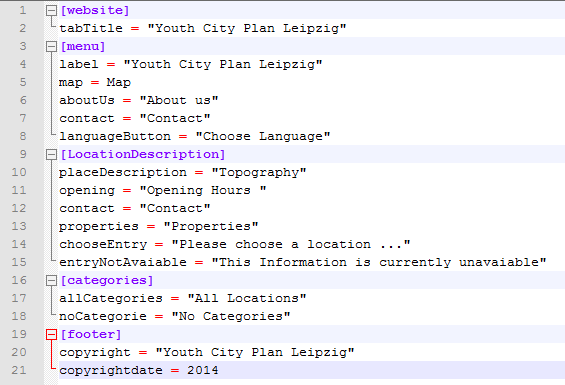
\includegraphics[width=.6\textwidth]{Screenshot.png}
  \end{center}
\end{itemize}

\section{Änderungen}

12.02.2015, HGG. Folgende Änderungen wurde vorgenommen:
\begin{itemize}
\item Umgang mit der Spracheinstellung: Statt
  \texttt{validateLanguage(language)} wird dies nun lokal, wo dies benötigt
  wird, durch einen Aufruf von \texttt{getLanguage()} realisiert.  Diese neue
  Funktion ist in \texttt{translate.php} definiert, womit \texttt{helper.php}
  obsolet ist und gelöscht wurde.
\item \texttt{buildHTMLPage.php} wurde nach \texttt{index.php} verschoben und
  entsprechend modifiziert, da weitere Webseiten einen ähnlichen Aufbau haben.
  Damit ist auch die Funktion \texttt{pageTemplate()} überflüssig und wurde
  gelöscht. 
\item Einheitliche Datenquelle ist das Verzeichnis \texttt{data/rdf}.  Das war
  in \texttt{custom-map.js} anzupassen. Das zweite Verzeichnis
  \texttt{public/data} wurde gelöscht.
\item Das Verzeichnis \texttt{data/rdf} enthält weiterhin ein Skript
  \texttt{trans.php}, mit dem eine JSON-RDF-Datei in eine Turtle-Datei
  verwandelt werden kann.  Damit wurde aus dem Original
  \texttt{jugendstadtplan.json} die Turtle-Datei \texttt{JSP-13.ttl} erzeugt,
  dort die fehlende Information für die Kategorie jsp:Bildung nachgetragen und
  das Ganze in eine neue Version der RDF-JSON-Datei
  \texttt{jugendstadtplan.json} zurückverwandelt.  Es zeigt sich in der
  Anwendung, dass EasyRDF solche RDF-JSON-Dateien deutlich schneller lädt als
  die entsprechende Turtle-Datei. 
\end{itemize}
\end{document}
